% Here we have your executive summary.

Your executive summary will give a detailed summary of your thesis, hitting the high points and perhaps including a figure or two.  This should have all of the important take-home messages; though details will of course be left for the thesis itself, here you should give enough detail for a reader to have a good idea of the content of the full document.  Importantly, this summary should be able to stand alone, separate from the rest of the document, so although you will be emphasizing the key results of your work, you will probably also want to include a sentence or two of introduction and context for the work you have done.

\begin{figure}[h!]
    \centering
    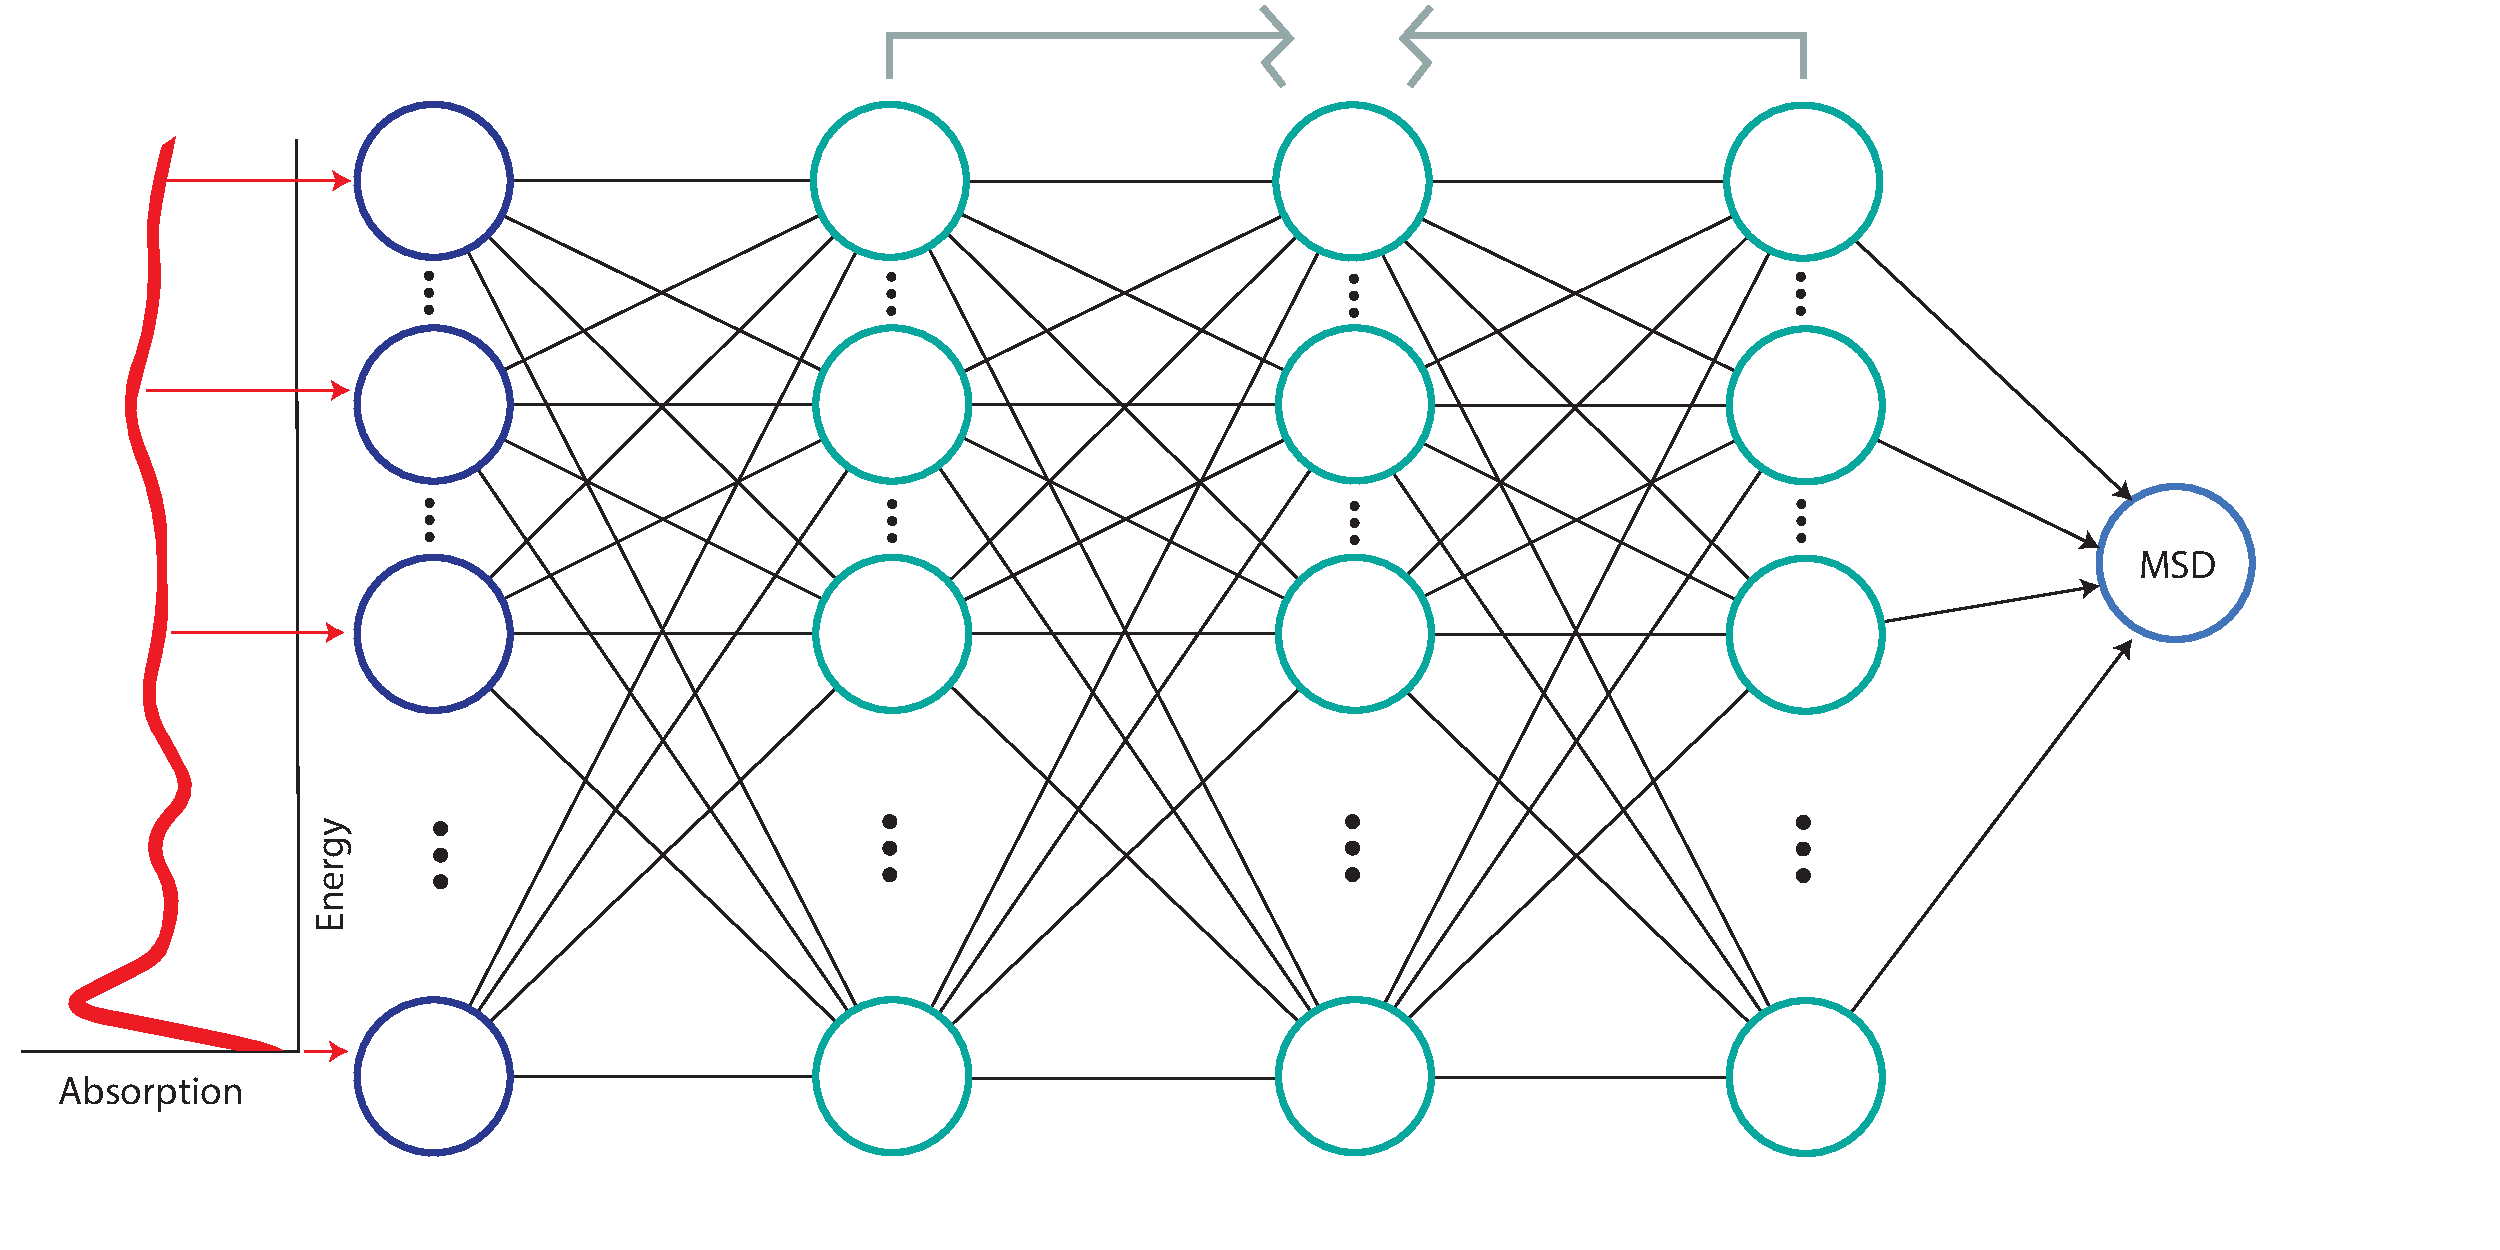
\includegraphics[width=\linewidth]{Chapters/Figures/thesis-design.pdf}
    \caption[Project Approach]{Thesis design}
\end{figure}
